\section{Experiments}

\begin{itemize}
  \item Fast neural Style: pytorch + vgg19 setup.
  \item Emotion detection: FER
  \item face detection haar cascades
  \item 
\end{itemize}


\subsection{Face and emotion detection}

We used a traditional Haar-Cascade classifier to detect faces within the camera's frame. To test the accuracy and detection rate, we recorded 5 short videos, 400 frames in length each. These frames were used to test the time it took the classifier to produce a result, and the accuracy of these results for our camera's resolution and use-case. 

The features we are looking for in our frames are both faces and eye features, because we not only want to keep a person within the camera's frame, but we also want to pass a cropped photo of the person to the emotion detector, which performs best when both eyes are visible. 

Regarding emotion detection, we used the CNN provided by Octavio Arriaga \cite{DBLP:journals/corr/abs-1710-07557}. On their publication, they report 66\% accuracy on the FER dataset on their "sequential fully-CNN".

When training this on FERPlus, we simplified the number of classes to 5 as we found that the robot's behaviour was too erratic with more classes. Our chosen emotions are happiness, surprise, fear, sadness and anger.


We measure the performance of our face and emotion detection algorithms by how much time it takes for them to produce a result, as each passing frame affects the quality of the final product.

\subsection{Style Transfer}


We started by taking Karras' team StyleGAN2 network description and adapting it to run on the Raspberry Pi 4s hardware. 


The purpose of using Karras' model was to try to minimize the requirements for inference of a trained model following their architecture. Our logic was that minimizing the footprint of the model, inference would be fast enough to complete in real time for our robot. In our early testing, reducing the input images to even below 100 x 100 px produced a model that had an inference time of around 30 seconds per frame on the Raspberry Pi hardware. We decided that the optimizations required to make this model work at a more reasonable speed were outside of our expertise, as we quickly realized that it required a deeper understanding of the Raspberry Pi's hardware to make use of platform-specific instructions. 

We moved onto implementing Justin Johnson's solution on our platform. Jhonson's original publication used Lua with Torch packages to implement a feedforward neural network to improve the speed of the original Gatys et. al paper's results. This implementation takes around 50 milliseconds per frame on a 1200 x 630 pixel image, which seems promising. 

We translated Jhonson's network architecture to be used in Python with Pytorch 1.9. We noticed that, as Jhonson points out in his publication, changing instance normalization for batch normalization has a very sizeable impact on speed performance at the cost of very minimal visual performance, as seen in in an example on figure \ref{fig:norm_comp}. 


\begin{figure}[h]
    \centering
        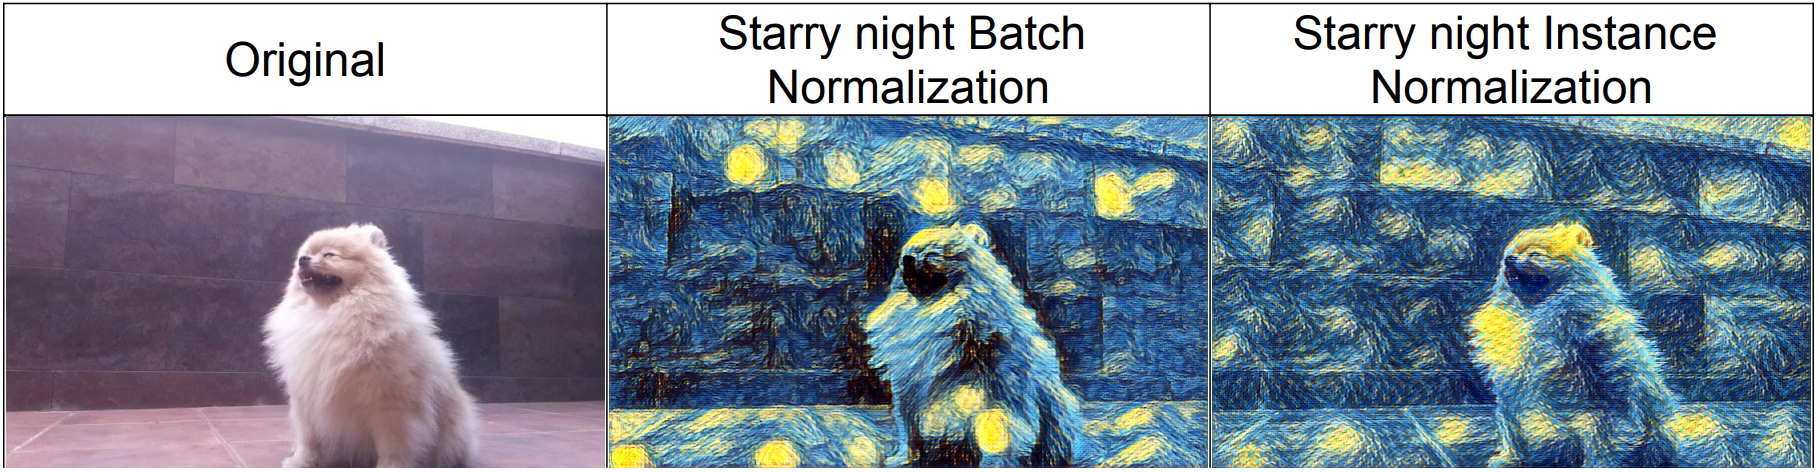
\includegraphics[width=\textwidth]{resources/style_norm_comp.png}        
        \caption{Comparison of instance vs batch normalization}
        \label{fig:norm_comp}
\end{figure}

More importantly, the average processing time for a frame using an instance normalization model was of 1.25 seconds, while batch normalization averaged 0.48 seconds per frame of processing time. 


\begin{figure}[h]
    \centering
        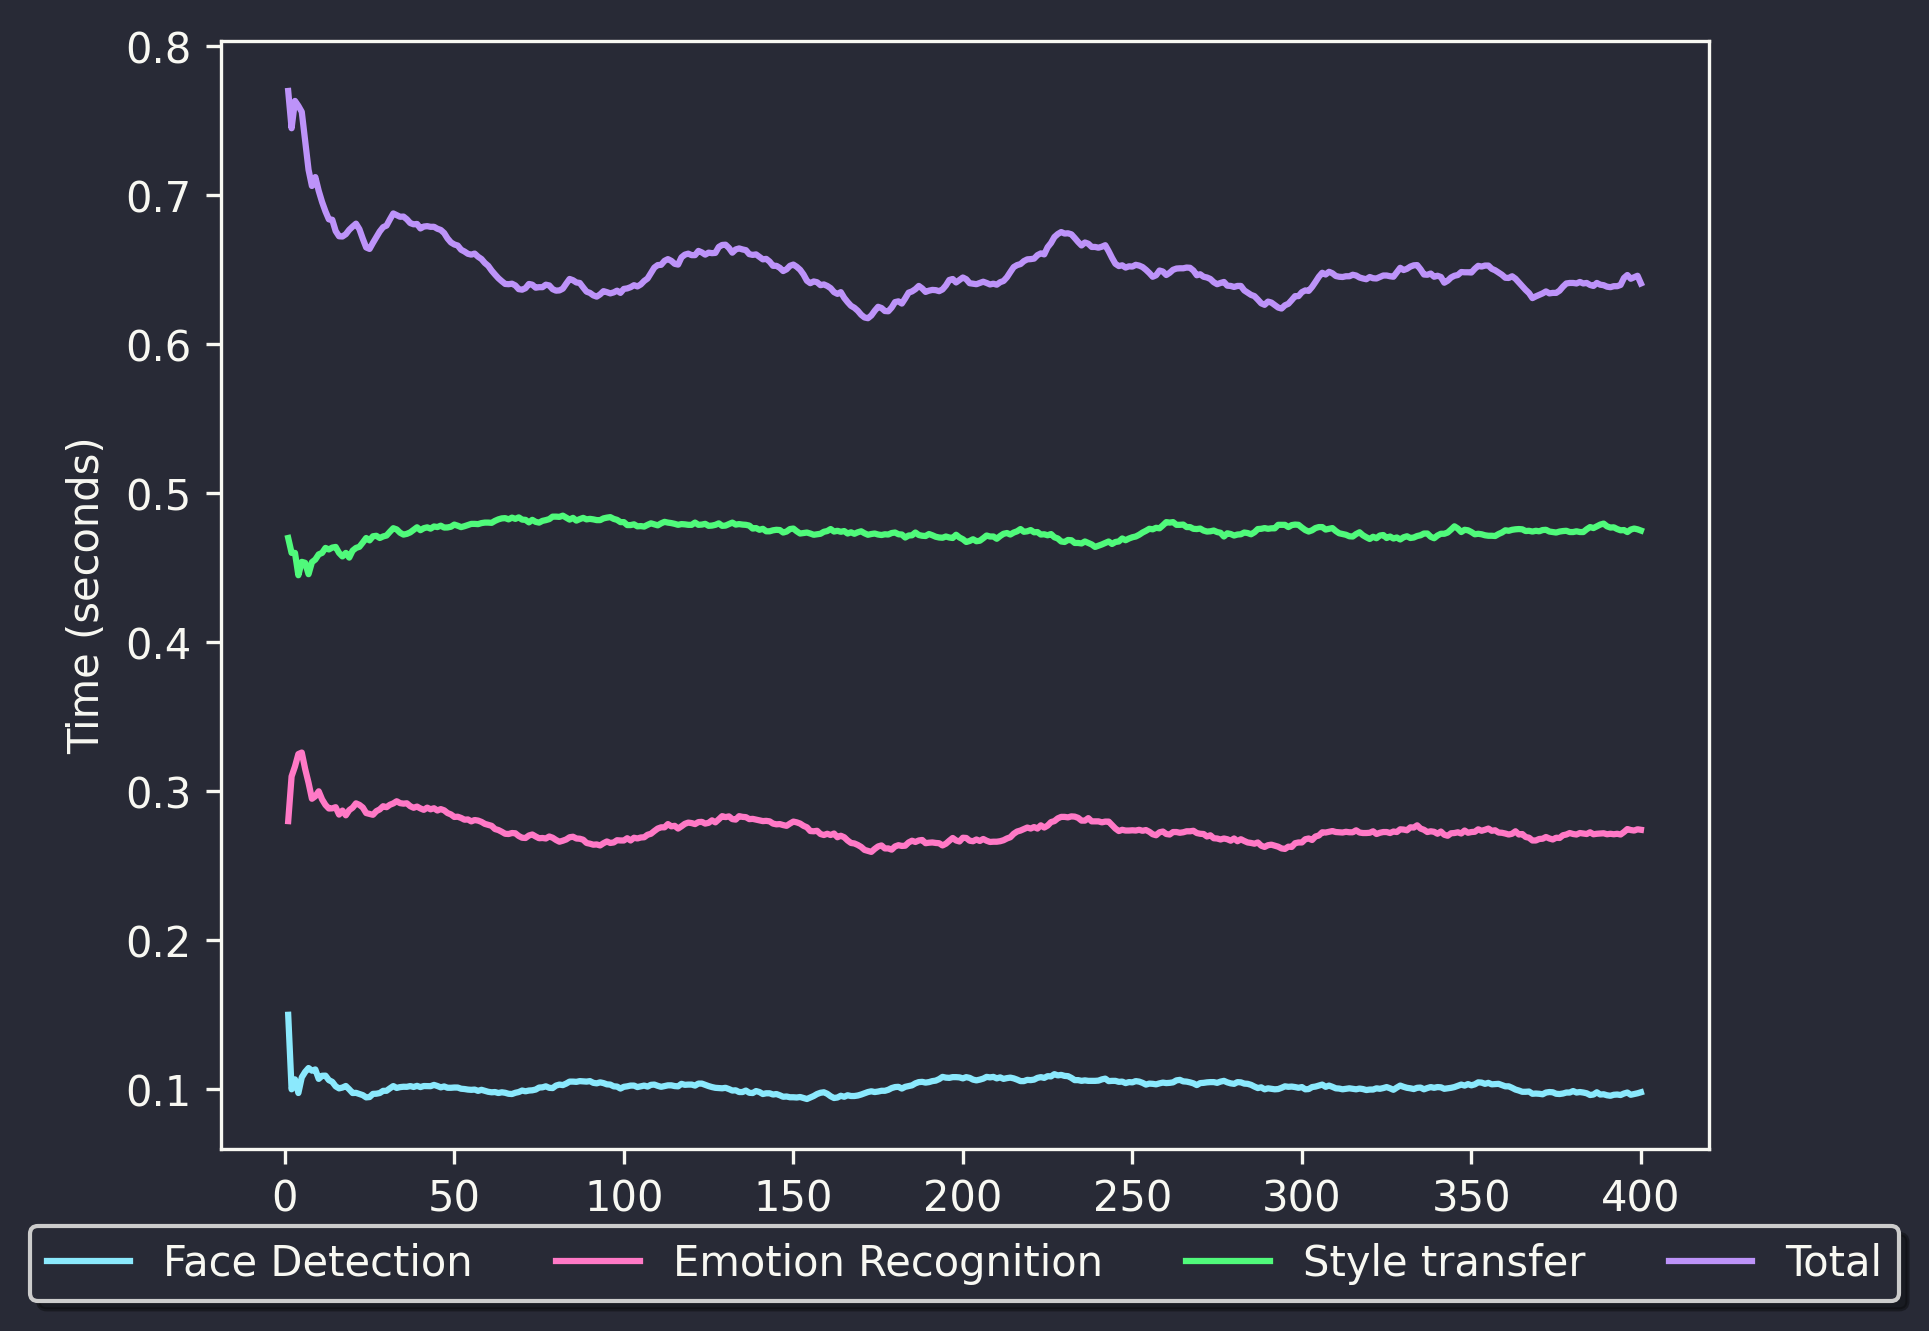
\includegraphics[width=\textwidth]{resources/total_frame_time.png}        
        \caption{Total time consumed per method each frame.}
        \label{fig:total_frame_time}
\end{figure}


\hl{TODO: fast neural style with vgg19}



\subsection{Robot state diagram}

\begin{figure}[h]
  \centering
  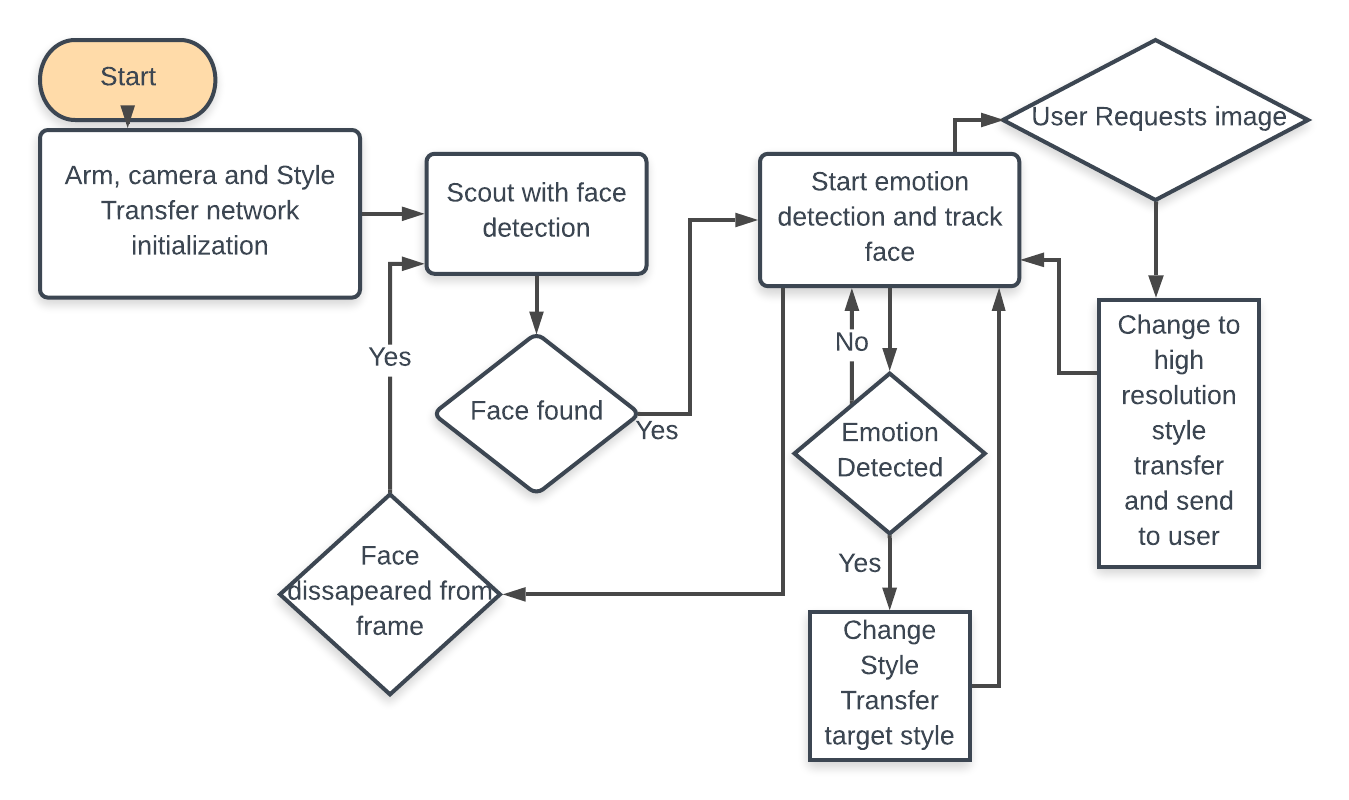
\includegraphics[width=\textwidth]{resources/state_machine.png}
  \caption{Robot flow diagram.}\label{fig:state_machine}
\end{figure}
